% Options for packages loaded elsewhere
% Options for packages loaded elsewhere
\PassOptionsToPackage{unicode}{hyperref}
\PassOptionsToPackage{hyphens}{url}
\PassOptionsToPackage{dvipsnames,svgnames,x11names}{xcolor}
%
\documentclass[
  13pt,
]{article}
\usepackage{xcolor}
\usepackage[margin=2cm]{geometry}
\usepackage{amsmath,amssymb}
\setcounter{secnumdepth}{5}
\usepackage{iftex}
\ifPDFTeX
  \usepackage[T1]{fontenc}
  \usepackage[utf8]{inputenc}
  \usepackage{textcomp} % provide euro and other symbols
\else % if luatex or xetex
  \usepackage{unicode-math} % this also loads fontspec
  \defaultfontfeatures{Scale=MatchLowercase}
  \defaultfontfeatures[\rmfamily]{Ligatures=TeX,Scale=1}
\fi
\usepackage{lmodern}
\ifPDFTeX\else
  % xetex/luatex font selection
  \setmainfont[]{Times New Roman}
\fi
% Use upquote if available, for straight quotes in verbatim environments
\IfFileExists{upquote.sty}{\usepackage{upquote}}{}
\IfFileExists{microtype.sty}{% use microtype if available
  \usepackage[]{microtype}
  \UseMicrotypeSet[protrusion]{basicmath} % disable protrusion for tt fonts
}{}
\usepackage{setspace}
\makeatletter
\@ifundefined{KOMAClassName}{% if non-KOMA class
  \IfFileExists{parskip.sty}{%
    \usepackage{parskip}
  }{% else
    \setlength{\parindent}{0pt}
    \setlength{\parskip}{6pt plus 2pt minus 1pt}}
}{% if KOMA class
  \KOMAoptions{parskip=half}}
\makeatother
% Make \paragraph and \subparagraph free-standing
\makeatletter
\ifx\paragraph\undefined\else
  \let\oldparagraph\paragraph
  \renewcommand{\paragraph}{
    \@ifstar
      \xxxParagraphStar
      \xxxParagraphNoStar
  }
  \newcommand{\xxxParagraphStar}[1]{\oldparagraph*{#1}\mbox{}}
  \newcommand{\xxxParagraphNoStar}[1]{\oldparagraph{#1}\mbox{}}
\fi
\ifx\subparagraph\undefined\else
  \let\oldsubparagraph\subparagraph
  \renewcommand{\subparagraph}{
    \@ifstar
      \xxxSubParagraphStar
      \xxxSubParagraphNoStar
  }
  \newcommand{\xxxSubParagraphStar}[1]{\oldsubparagraph*{#1}\mbox{}}
  \newcommand{\xxxSubParagraphNoStar}[1]{\oldsubparagraph{#1}\mbox{}}
\fi
\makeatother


\usepackage{longtable,booktabs,array}
\usepackage{calc} % for calculating minipage widths
% Correct order of tables after \paragraph or \subparagraph
\usepackage{etoolbox}
\makeatletter
\patchcmd\longtable{\par}{\if@noskipsec\mbox{}\fi\par}{}{}
\makeatother
% Allow footnotes in longtable head/foot
\IfFileExists{footnotehyper.sty}{\usepackage{footnotehyper}}{\usepackage{footnote}}
\makesavenoteenv{longtable}
\usepackage{graphicx}
\makeatletter
\newsavebox\pandoc@box
\newcommand*\pandocbounded[1]{% scales image to fit in text height/width
  \sbox\pandoc@box{#1}%
  \Gscale@div\@tempa{\textheight}{\dimexpr\ht\pandoc@box+\dp\pandoc@box\relax}%
  \Gscale@div\@tempb{\linewidth}{\wd\pandoc@box}%
  \ifdim\@tempb\p@<\@tempa\p@\let\@tempa\@tempb\fi% select the smaller of both
  \ifdim\@tempa\p@<\p@\scalebox{\@tempa}{\usebox\pandoc@box}%
  \else\usebox{\pandoc@box}%
  \fi%
}
% Set default figure placement to htbp
\def\fps@figure{htbp}
\makeatother


% definitions for citeproc citations
\NewDocumentCommand\citeproctext{}{}
\NewDocumentCommand\citeproc{mm}{%
  \begingroup\def\citeproctext{#2}\cite{#1}\endgroup}
\makeatletter
 % allow citations to break across lines
 \let\@cite@ofmt\@firstofone
 % avoid brackets around text for \cite:
 \def\@biblabel#1{}
 \def\@cite#1#2{{#1\if@tempswa , #2\fi}}
\makeatother
\newlength{\cslhangindent}
\setlength{\cslhangindent}{1.5em}
\newlength{\csllabelwidth}
\setlength{\csllabelwidth}{3em}
\newenvironment{CSLReferences}[2] % #1 hanging-indent, #2 entry-spacing
 {\begin{list}{}{%
  \setlength{\itemindent}{0pt}
  \setlength{\leftmargin}{0pt}
  \setlength{\parsep}{0pt}
  % turn on hanging indent if param 1 is 1
  \ifodd #1
   \setlength{\leftmargin}{\cslhangindent}
   \setlength{\itemindent}{-1\cslhangindent}
  \fi
  % set entry spacing
  \setlength{\itemsep}{#2\baselineskip}}}
 {\end{list}}
\usepackage{calc}
\newcommand{\CSLBlock}[1]{\hfill\break\parbox[t]{\linewidth}{\strut\ignorespaces#1\strut}}
\newcommand{\CSLLeftMargin}[1]{\parbox[t]{\csllabelwidth}{\strut#1\strut}}
\newcommand{\CSLRightInline}[1]{\parbox[t]{\linewidth - \csllabelwidth}{\strut#1\strut}}
\newcommand{\CSLIndent}[1]{\hspace{\cslhangindent}#1}



\setlength{\emergencystretch}{3em} % prevent overfull lines

\providecommand{\tightlist}{%
  \setlength{\itemsep}{0pt}\setlength{\parskip}{0pt}}



 


\usepackage[noblocks]{authblk}
% packages needed by kableExtra tables (not recorded when chunks are cached)
\usepackage{float}
% blinded: empty author, otherwise authblk prints the word "immediate"
\author{}
\usepackage{multirow}
\usepackage{colortbl}
\renewcommand*{\Authsep}{, }
\renewcommand*{\Authand}{, }
\renewcommand*{\Authands}{, }
\renewcommand\Affilfont{\small}
\makeatletter
\@ifpackageloaded{caption}{}{\usepackage{caption}}
\AtBeginDocument{%
\ifdefined\contentsname
  \renewcommand*\contentsname{Table of contents}
\else
  \newcommand\contentsname{Table of contents}
\fi
\ifdefined\listfigurename
  \renewcommand*\listfigurename{List of Figures}
\else
  \newcommand\listfigurename{List of Figures}
\fi
\ifdefined\listtablename
  \renewcommand*\listtablename{List of Tables}
\else
  \newcommand\listtablename{List of Tables}
\fi
\ifdefined\figurename
  \renewcommand*\figurename{Figure}
\else
  \newcommand\figurename{Figure}
\fi
\ifdefined\tablename
  \renewcommand*\tablename{Table}
\else
  \newcommand\tablename{Table}
\fi
}
\@ifpackageloaded{float}{}{\usepackage{float}}
\floatstyle{ruled}
\@ifundefined{c@chapter}{\newfloat{codelisting}{h}{lop}}{\newfloat{codelisting}{h}{lop}[chapter]}
\floatname{codelisting}{Listing}
\newcommand*\listoflistings{\listof{codelisting}{List of Listings}}
\makeatother
\makeatletter
\makeatother
\makeatletter
\@ifpackageloaded{caption}{}{\usepackage{caption}}
\@ifpackageloaded{subcaption}{}{\usepackage{subcaption}}
\makeatother
\usepackage{bookmark}
\IfFileExists{xurl.sty}{\usepackage{xurl}}{} % add URL line breaks if available
\urlstyle{same}
\hypersetup{
  pdftitle={Do meritocratic beliefs undermine the acceptance of privilege at school-age? A longitudinal equivalence approach},
  colorlinks=true,
  linkcolor={blue},
  filecolor={Maroon},
  citecolor={Blue},
  urlcolor={Blue},
  pdfcreator={LaTeX via pandoc}}


\title{Do meritocratic beliefs undermine the acceptance of privilege at
school-age? A longitudinal equivalence approach}



\date{}
\begin{document}
\maketitle
\begin{abstract}
Schools are key spaces of meritocratic socialization, shaping students'
understanding of whether success is earned or inherited. Yet little is
known about how students conceive meritocracy and how these conceptions
relate to the acceptance of privilege. This study examines whether
perceptions and preferences about meritocracy and privilege form
distinct yet related dimensions of students' beliefs, and how they
change over time and across school stages. Using a novel instrument
previously applied to adults, we surveyed Chilean students in 6th and
9th grade (Wave 1: N = 846) and again in 7th and 10th grade (Wave 2: N =
662). Results support a multidimensional organization of beliefs:
endorsing meritocratic criteria can coexist with accepting privilege
rather than displacing it. Older students also judge more critically
whether effort is rewarded. These findings suggest that such beliefs are
shaped early in socialization but shift in a critical direction as
students mature.

\textbf{Keywords}: Meritocracy · Privilege · Schools · Measurement
invariance · Socialization · Chile

\textbf{Word count}: 7,850 (main text, tables, captions, statements and
references; abstract excluded)
\end{abstract}


\setstretch{1.5}
\section{Introduction}\label{introduction}

The way in which children and youths come to understand who succeeds in
society and why is a relevant aspect of the socialization process
(\citeproc{ref-mijs_unfulfillable_2016}{Mijs, 2016};
\citeproc{ref-resh_sense_2014}{Resh \& Sabbagh, 2014}). Schools are
important actors in this regard, as they use grading, tracking, and
selection to apply meritocratic criteria based primarily on individual
talent and effort (\citeproc{ref-darnon_where_2018}{Darnon et al.,
2018}; \citeproc{ref-traini_stratification_2022}{Traini, 2022}). This
early exposure to meritocratic principles in the ``impressionable
years'' (\citeproc{ref-krosnick_aging_1989}{Krosnick \& Alwin, 1989})
shapes students' understanding of fairness, social mobility, and social
hierarchies. At the same time, schools are environments where students
encounter evidence that outcomes are shaped by factors other than
meritocratic ones, such as family background, social connections, and
structural advantages usually associated with privilege
(\citeproc{ref-bourdieu_reproduction_1990}{Bourdieu \& Passeron, 1990};
\citeproc{ref-goudeau_hidden_2017a}{Goudeau \& Croizet, 2017};
\citeproc{ref-tang_meritocratic_2025}{Tang et al., 2025}). These
background attributes can be considered privileges due to heritage-based
advantages over which people have no control, unlike effort. Yet, few
studies have explored how students conceive meritocracy and to what
extent such conceptions challenge the role of privilege in society.

Although meritocracy is often treated as a single dimension, mostly
related to individual effort, the literature increasingly suggests that
it is a multidimensional construct. On the one hand, this refers to the
distinction between perceptions of how meritocracy operates in society
(``what is'') and preferences about how it should operate (``what ought
to be'') (\citeproc{ref-castillo_multidimensional_2023}{Castillo et al.,
2023}; \citeproc{ref-duru-bellat_whos_2012}{Duru-Bellat \& Tenret,
2012}). On the other hand, meritocratic beliefs can be distinguished
from privilege-based beliefs, which emphasize the role of family wealth
and social connections in shaping rewards in society
(\citeproc{ref-liu_does_2025}{C. Liu \& Wang, 2025};
\citeproc{ref-tang_meritocratic_2025}{Tang et al., 2025}). A
multidimensional approach should therefore incorporate perceptions and
preferences about both meritocratic and privilege-based explanations of
social outcomes, in line with Khan's
(\citeproc{ref-khan_privilege_2013}{2013}) call to analyze meritocracy
together with privilege.

Previous research has shown that privilege and meritocratic beliefs
represent different and not necessarily opposite dimensions, therefore
they can coexist in people's minds
(\citeproc{ref-fan_disillusionment_2026}{Fan et al., 2026};
\citeproc{ref-liu_does_2025}{C. Liu \& Wang, 2025};
\citeproc{ref-tang_meritocratic_2025}{Tang et al., 2025}). This means,
for instance, that someone could believe that society rewards talent and
effort while also acknowledging that family wealth and social
connections play (or should play) a role in shaping outcomes. However,
attempts to study these beliefs have been limited by the lack of
instruments that capture their multidimensionality and by the absence of
longitudinal studies that examine how these beliefs evolve over time. We
contribute to this agenda by applying a multidimensional model to
measure meritocratic and privilege beliefs in a sample of Chilean
students and by examining the stability and measurement equivalence of
these beliefs across school stages and over time. We argue that
meritocratic and privilege beliefs can be distinguished even at an early
school age, with a structure similar to that found among adults
(\citeproc{ref-castillo_multidimensional_2023}{Castillo et al., 2023});
that they are not two ends of the same continuum but can coexist in
students' minds; and that they are not static but evolve as students
gain experience and exposure to different social contexts.

We draw on a two-wave panel of Chilean students in primary and secondary
school cohorts. Chile's educational system combines high stratification,
market-based competition, and explicit meritocratic discourse in school
culture (\citeproc{ref-castillo_socialization_2024}{Castillo et al.,
2024}; \citeproc{ref-valenzuela_socioeconomic_2013}{Valenzuela et al.,
2013}), alongside persistent socioeconomic inequality and a deep
marketization of social welfare
(\citeproc{ref-ferre_welfare_2023}{Ferre, 2023};
\citeproc{ref-madariaga_three_2020}{Madariaga, 2020}), features shared
by many Latin American countries and increasingly present in European
and East Asian systems (\citeproc{ref-busemeyer_skills_2014}{Busemeyer,
2014}; \citeproc{ref-gingrich_making_2011}{Gingrich, 2011}). This makes
Chile a productive case for studying how students internalize, question,
or reconcile meritocratic ideals with the reality of privilege, while
the dimensional structure and longitudinal patterns identified here are
likely to travel to other highly stratified educational contexts.

The research questions guiding this study are as follows:

\begin{enumerate}
\def\labelenumi{(\arabic{enumi})}
\item
  Are school-aged students able to distinguish between meritocratic and
  privilege-based principles, as well as between perceptions (``what
  is'') and preferences (``what should be'')?
\item
  Are meritocratic beliefs undermined (i.e., negatively associated) by
  beliefs about privilege, or could they coexist in students' minds?
\item
  Are these dimensions stable over time and across school stages?
\end{enumerate}

\section{Theoretical and empirical
background}\label{theoretical-and-empirical-background}

\subsection{The socialization of meritocracy at
school}\label{the-socialization-of-meritocracy-at-school}

Meritocracy refers to a distributive system in which individual merit,
typically defined as effort and personal ability, is treated as the
primary criterion for allocating resources and rewards, rather than
social origins or inherited privilege
(\citeproc{ref-young_rise_1958}{Young, 1958}). While Young
(\citeproc{ref-young_rise_1958}{1958}) coined the term as a dystopian
critique, it has since been re-appropriated as a positive ideal of
fairness in liberal and market-oriented societies
(\citeproc{ref-mijs_paradox_2021}{Mijs, 2021};
\citeproc{ref-vandewerfhorst_meritocracy_2024}{Van De Werfhorst, 2024}).
From a sociological standpoint, meritocracy operates both as a cognitive
judgment about how inequality works and as a moral lens through which
people evaluate whether unequal outcomes are deserved
(\citeproc{ref-heuer_legitimizing_2020}{Heuer et al., 2020}). Because it
frames outcomes as earned, meritocracy can reinforce inequality:
``winners'' see their position as deserved, while ``losers'' are pushed
toward self-blame rather than structural critique
(\citeproc{ref-garcia-sierra_dark_2023}{García-Sierra, 2023};
\citeproc{ref-sandel_tyranny_2020}{Sandel, 2020}). In this line,
research in adult populations has documented systematic associations
between meritocratic beliefs and the justification of social
inequalities (\citeproc{ref-liu_does_2025}{C. Liu \& Wang, 2025};
\citeproc{ref-mijs_paradox_2021}{Mijs, 2021};
\citeproc{ref-tejero-peregrina_perceived_2025}{Tejero-Peregrina et al.,
2025}). Yet how and when these beliefs develop, and whether they can be
identified at early stages of socialization, has received little
attention.

Schools are key institutions when it comes to the socialization of
meritocracy. On the one hand, they advance meritocratic ideals through
narratives of effort, achievement, self-improvement, and education as a
legitimate route to rewards and social mobility
(\citeproc{ref-batruch_belief_2022}{Batruch et al., 2022};
\citeproc{ref-chauvin_school_2026}{Chauvin et al., 2026};
\citeproc{ref-darnon_where_2018}{Darnon et al., 2018};
\citeproc{ref-wiederkehr_belief_2015}{Wiederkehr et al., 2015}). On the
other hand, they embed these ideals in routine practices of grading,
tracking, selection, awards, and credentialing, which operate as
institutional markers of worth that make merit visible and consequential
in ways that are immediate and socially meaningful
(\citeproc{ref-resh_sense_2014}{Resh \& Sabbagh, 2014};
\citeproc{ref-traini_stratification_2022}{Traini, 2022}). At the same
time, schools are also settings where privilege-based advantages,
including family resources, cultural capital, peer environments, and
unequal school quality, are also visible and consequential
(\citeproc{ref-batruch_belief_2022}{Batruch et al., 2022};
\citeproc{ref-bernstein_pedagogy_1996}{Bernstein, 1996};
\citeproc{ref-goudeau_hidden_2017a}{Goudeau \& Croizet, 2017};
\citeproc{ref-khan_saying_2013}{Khan \& Jerolmack, 2013};
\citeproc{ref-lareau_unequal_2003}{Lareau, 2003}). Students may endorse
meritocracy as a normative ideal while simultaneously recognizing
structural constraints, reflecting what the literature describes as dual
consciousness (\citeproc{ref-kluegel_beliefs_1987}{Kluegel \& Smith,
1987}; \citeproc{ref-liu_does_2025}{C. Liu \& Wang, 2025};
\citeproc{ref-tang_meritocratic_2025}{Tang et al., 2025}).

The dynamics of the socialization of meritocracy can change over time.
Developmental research suggests that by around age 10, children already
articulate judgments about social differences, typically emphasizing
individual, merit-based explanations while only beginning to incorporate
opportunity-based accounts (\citeproc{ref-imhoff_nociones_2025}{Imhoff
\& Brussino, 2025}; \citeproc{ref-sigelman_age_2013a}{Sigelman, 2013}).
As students move through the school system, however, cumulative exposure
to grading, tracking, peer comparison, and visible socioeconomic gaps
can make the limits of effort as a sufficient explanation for success
increasingly apparent. Tang et al.
(\citeproc{ref-tang_meritocratic_2025}{2025}) show that among Chinese
college students, those from lower socioeconomic backgrounds initially
report lower recognition of privilege-based advantages than their
higher-SES peers, but this gap narrows progressively across college
years as both groups converge toward stronger acknowledgment of
structural advantage. This suggests not simply that older students
believe less in meritocracy, but that sustained exposure to the
educational system makes structural advantage harder to ignore
--referred to as the ``reality shock''
(\citeproc{ref-allen_top_2016}{Allen, 2016}). Adolescence is therefore a
particularly consequential period for studying these processes,
precisely when abstract reasoning about justice and fairness becomes
more sophisticated and school-based sorting mechanisms grow more salient
(\citeproc{ref-henry_development_2006}{Henry \& Saul, 2006};
\citeproc{ref-resh_sense_2014}{Resh \& Sabbagh, 2014}).

\subsection{Conceptualizing and measuring meritocratic and privilege
beliefs}\label{conceptualizing-and-measuring-meritocratic-and-privilege-beliefs}

Most attempts to operationalize meritocratic beliefs often follow
Young's (\citeproc{ref-young_rise_1958}{1958}) formulation (Merit =
Effort + Intelligence). For instance, the ``Preference for the Merit
Principle Scale'' (\citeproc{ref-davey_preference_1999}{Davey et al.,
1999}) and the ``Belief in School Meritocracy Scale''
(\citeproc{ref-batruch_belief_2022}{Batruch et al., 2022}) focus on the
perceived importance of effort and ability for success, while Wiederkehr
et al. (\citeproc{ref-wiederkehr_belief_2015}{2015}) measure the extent
to which respondents believe that hard work is rewarded. These
approaches, however, risk conflating meritocratic beliefs with general
attitudes toward effort or achievement, potentially overlooking the
broader structural and relational dimensions of meritocracy. Other
approaches treat meritocratic beliefs as interchangeable with constructs
such as system justification (\citeproc{ref-jost_decade_2004a}{Jost et
al., 2004}), beliefs about social mobility
(\citeproc{ref-deng_its_2025}{Deng \& Wang, 2025}), or generalized
support for equal opportunity
(\citeproc{ref-batruch_belief_2022}{Batruch et al., 2022};
\citeproc{ref-darnon_where_2018}{Darnon et al., 2018}).

A further limitation in the conceptualization of meritocratic beliefs
concerns privilege-based factors such as family wealth, social
connections, and other structural advantages
(\citeproc{ref-khan_saying_2013}{Khan \& Jerolmack, 2013}). As Castillo
et al. (\citeproc{ref-castillo_multidimensional_2023}{2023}) notes, much
survey research relies on item batteries that ask respondents to rate
the importance of effort, talent, family background, networks, or luck
for ``getting ahead'', and then reduces these into a single score. This
becomes especially problematic when researchers construct continuum
measures in composite indicators, treating meritocratic and
privilege-based explanations as opposite ends of the same scale (e.g.,
by subtracting ``non-merit'' from ``merit,'' as in
\citeproc{ref-reynolds_perceptions_2014}{Reynolds \& Xian, 2014}). Such
operationalizations embed a strong zero-sum assumption, namely that
endorsing merit necessarily entails rejecting structural or relational
advantages, thereby ruling out, by design, the empirical possibility
that both types of beliefs coexist. Recent debates, including the
exchange between Mijs (\citeproc{ref-mijs_visualizing_2026}{2026}) and
Wiesner \& Sachweh (\citeproc{ref-wiesner_effort_2026}{2026}),
underscore this point by arguing for measures that capture meritocratic
beliefs alongside privilege-based ones, rather than as a residual of the
relative importance assigned to structural factors. Empirical work
points in the same direction: meritocratic endorsement may remain stable
as recognition of structural constraints increases
(\citeproc{ref-liu_does_2025}{C. Liu \& Wang, 2025};
\citeproc{ref-tang_meritocratic_2025}{Tang et al., 2025}), support for
merit can coexist with recognition of social connections in distinct
attitudinal clusters (\citeproc{ref-kwon_multidimensionality_2024}{Kwon
\& Pandian, 2024}), and meritocratic and structural explanations often
accumulate rather than replace one another
(\citeproc{ref-zhu_meritocratic_2025}{Zhu, 2025}). Unidimensional
indices, and especially subtraction scores, can therefore manufacture
artificial neutral positions and blur substantively distinct belief
profiles that could hide relevant group differences and changes over
time.

In response to the previously mentioned limitations, Castillo et al.
(\citeproc{ref-castillo_multidimensional_2023}{2023}) proposed a
multidimensional framework that decomposes meritocratic beliefs along
two analytically independent axes: perceptions (what is) versus
preferences (what ought to be), and meritocratic versus privilege-based
(originally called ``non-meritocratic'') allocation principles.
Meritocratic elements (effort, talent) and privilege-based elements
(family wealth, networks) are treated as distinct components rather than
as opposites. This yields four separate constructs, allowing belief
combinations that older measures tend to collapse, such as endorsing
meritocracy as an ideal while simultaneously recognizing the weight of
family background and connections (\citeproc{ref-khan_saying_2013}{Khan
\& Jerolmack, 2013}). Evidence from adult samples using confirmatory
factor analysis supports a four-factor structure (perceptions and
preferences of both meritocracy and privilege)
(\citeproc{ref-castillo_multidimensional_2023}{Castillo et al., 2023}),
a pattern that aligns with Zhu's
(\citeproc{ref-zhu_meritocratic_2025}{2025}) notion of dual
consciousness, here understood as the simultaneous endorsement of
meritocracy as a normative ideal alongside descriptive recognition that
rewards are shaped by structural advantage.

Attention to measurement quality, through confirmatory factor analysis
and measurement invariance, is not merely a technical concern. As the
sociological discussion on \emph{estimands}
(\citeproc{ref-lundberg_what_2021}{Lundberg et al., 2021}) stresses,
constructs must be theoretically meaningful and empirically
identifiable; otherwise, conclusions may reflect artifacts of
measurement rather than substantive social phenomena. Invariance
analysis assesses whether the same latent construct is measured across
groups or over time, a precondition for valid comparisons and
developmental inference (\citeproc{ref-davidov_measurement_2014}{Davidov
et al., 2014}; \citeproc{ref-leitgob_measurement_2023}{Leitgöb et al.,
2023}; \citeproc{ref-putnick_measurement_2016}{Putnick \& Bornstein,
2016}). Beyond establishing comparability, it identifies which aspects
of a construct are equivalent and which are not, which is particularly
relevant for students' meritocratic and privilege beliefs, whose
socialization may change over time and across school stages
(\citeproc{ref-liu_does_2025}{C. Liu \& Wang, 2025};
\citeproc{ref-tang_meritocratic_2025}{Tang et al., 2025}).

Building on the previous background, we state the following hypotheses:

\textbf{\(H_1\) (Dimensional differentiation)}: Students' meritocratic
and privilege beliefs can be represented and measured by four distinct
dimensions: perceived meritocracy, perceived privilege, meritocratic
preferences, and privilege acceptance.

\textbf{\(H_2\) (Beliefs compatibility)}: merit and privilege beliefs
are not mutually exclusive, but rather compatible orientations that can
coexist within the same individual. This means that endorsing merit does
not necessarily imply rejection of privilege.

\textbf{\(H_3\) (Equivalence)}: The four-factor model is equivalent
across the two waves of the panel survey and across two student cohorts
-- 6th and 9th grade (or first-year secondary) in the first wave.

\section{Methods}\label{methods}

\subsection{Participants}\label{participants}

This study uses secondary data from the 2023 and 2024 waves of a panel
survey on education and meritocracy {[}name withheld for anonymous
review{]}. The panel examines school-age students' beliefs, attitudes,
and behaviors regarding meritocracy, inequality, and citizenship.

The questionnaire was administered to sixth-grade and ninth-grade
students (primary and secondary cohorts, respectively) in nine schools
in Chile's Metropolitan and Valparaíso regions. Although the sample was
non-probabilistic and lacked quota controls, a minimum target of 900
students was set to ensure adequate statistical power. After data
processing and listwise deletion, the analytical sample included 846
students in Wave 1 and 662 in Wave 2 (see Table~\ref{tbl-cohort} for age
and gender by cohort), yielding a retention rate of 78.3\% (attrition =
21.7\%). The main sources of attrition were school transfers between
academic years and high absenteeism in several schools.

\begin{table}[H]

\caption{\label{tbl-cohort}Descriptive statistics for cohort level}

\centering{

\centering\begingroup\fontsize{9.5}{11.5}\selectfont

\resizebox{\ifdim\width>\linewidth\linewidth\else\width\fi}{!}{
\begin{tabular}{>{\raggedright\arraybackslash}p{1.8cm}>{\raggedright\arraybackslash}p{2.2cm}>{\raggedleft\arraybackslash}p{1.6cm}>{\raggedleft\arraybackslash}p{1.6cm}>{\raggedleft\arraybackslash}p{1.6cm}>{\raggedleft\arraybackslash}p{1.9cm}>{\raggedleft\arraybackslash}p{1.9cm}>{\raggedleft\arraybackslash}p{1.9cm}}
\toprule
\multicolumn{3}{c}{ } & \multicolumn{2}{c}{Age} & \multicolumn{3}{c}{Gender} \\
\cmidrule(l{3pt}r{3pt}){4-5} \cmidrule(l{3pt}r{3pt}){6-8}
Wave & level & N & Mean & SD & Man & Women & Others\\
\midrule
 & Primary & 406 & 11.85 & 0.56 & 195 & 191 & 20\\
\cmidrule{2-8}
 & Secondary & 440 & 14.79 & 0.80 & 226 & 195 & 19\\
\cmidrule{2-8}
\multirow{-3}{1.8cm}{\raggedright\arraybackslash Wave 1} & Total & 846 & 13.38 & 1.63 & 421 & 386 & 39\\
\cmidrule{1-8}
 & Primary & 319 & 12.83 & 0.55 & 161 & 145 & 13\\
\cmidrule{2-8}
 & Secondary & 343 & 15.76 & 0.75 & 177 & 158 & 8\\
\cmidrule{2-8}
\multirow{-3}{1.8cm}{\raggedright\arraybackslash Wave 2} & Total & 662 & 14.35 & 1.61 & 338 & 303 & 21\\
\bottomrule
\end{tabular}}
\endgroup{}

}

\end{table}%

\subsection{Procedure}\label{procedure}

Data were collected by a professional research firm using a
Computer-Assisted Web Interviewing (CAWI) approach, based on online
questionnaires. Written informed consent was obtained for all
participants: students signed the consent form, which was reviewed and
approved by a parent or legal guardian, and only students with signed
consent were included in the study. To enable longitudinal linkage while
protecting confidentiality, the survey firm generated anonymous unique
identifiers for each student, and no directly identifying information
was included in the analytic files. The analytic code and data are
available as described in the data availability statement.

The study was approved by the Research Ethics Committee of
{[}institution withheld for anonymous review{]} (reference number
withheld for anonymous review), which determined that the project posed
minimal risk and approved the consent and confidentiality procedures.

\subsection{Measures}\label{measures}

\subsubsection{Perceptions and preferences of meritocracy and
privilege}\label{perceptions-and-preferences-of-meritocracy-and-privilege}

Meritocratic and privilege-based perceptions and preferences were
measured with the eight items of the original scale
(\citeproc{ref-castillo_multidimensional_2023}{Castillo et al., 2023}),
two per dimension :

\begin{itemize}
\item
  Meritocratic perceptions: the extent to which effort and ability are
  rewarded in Chile,
\item
  Privilege perceptions: the extent to which success is perceived as
  linked to connections and family wealth,
\item
  Meritocratic preferences: agreement that those who work harder or are
  more talented should be better rewarded,
\item
  Privilege acceptance: agreement that it is acceptable for individuals
  with better connections or wealthy parents to achieve greater success.
\end{itemize}

Each item (see Table~\ref{tbl-merit}) is rated on a four-point scale
ranging from ``strongly disagree'' (1) to ``strongly agree'' (4); higher
scores indicate stronger endorsement of the corresponding perception or
preference. The original Spanish wording of the items is reported in the
supplementary material.

\begin{table}[H]

\caption{\label{tbl-merit}Items for perceptions and preferences for
meritocracy scale}

\centering{

\centering\begingroup\fontsize{9.5}{11.5}\selectfont

\resizebox{\ifdim\width>\linewidth\linewidth\else\width\fi}{!}{
\begin{tabular}{>{\raggedright\arraybackslash}p{2cm}>{\raggedright\arraybackslash}p{2 cm}>{\raggedright\arraybackslash}p{10cm}}
\toprule
Components & Dimensions & Item\\
\midrule
 &  & In Chile people are rewarded for their efforts\\
\cmidrule{3-3}
 & \multirow{-2}{2 cm}{\raggedright\arraybackslash Meritocratic} & In Chile people are rewarded for their intelligence and ability\\
\cmidrule{2-3}
 &  & In Chile those with wealthy parents do much better in life\\
\cmidrule{3-3}
\multirow{-4}{2cm}[0.5\dimexpr\aboverulesep+\belowrulesep+\cmidrulewidth]{\raggedright\arraybackslash Perception} & \multirow{-2}{2 cm}{\raggedright\arraybackslash Privilege} & In Chile those with good contacts do much better in life\\
\cmidrule{1-3}
 &  & Those who work harder should reap greater rewards than those who work less hard\\
\cmidrule{3-3}
 & \multirow{-2}{2 cm}{\raggedright\arraybackslash Meritocratic} & Those with more talent should reap greater rewards than those with less talent\\
\cmidrule{2-3}
 &  & It is good that those who have rich parents do better in life\\
\cmidrule{3-3}
\multirow{-4}{2cm}[0.5\dimexpr\aboverulesep+\belowrulesep+\cmidrulewidth]{\raggedright\arraybackslash Preference} & \multirow{-2}{2 cm}{\raggedright\arraybackslash Privilege} & It is good that those who have good contacts do better in life\\
\bottomrule
\end{tabular}}
\endgroup{}

}

\end{table}%

\subsection{Analytical strategy}\label{analytical-strategy}

\subsubsection{Measurement model and
estimation}\label{measurement-model-and-estimation}

We estimated a Confirmatory Factor Analysis (CFA) with four latent
factors, using Diagonally Weighted Least Squares with robust correction
(WLSMV), which is suitable for ordinal items
(\citeproc{ref-kline_principles_2023}{Kline, 2023}). Model fit was
assessed following the guidelines of Brown
(\citeproc{ref-brown_confirmatory_2015}{2015}), using several indices:
the Comparative Fit Index (CFI) and the Tucker-Lewis Index (TLI), with
acceptable values above 0.95; the Root Mean Square Error of
Approximation (RMSEA), with values below 0.06 indicating good fit; and
the Chi-square statistic (acceptable fit indicated by \(p\)
\textgreater{} 0.05 and a Chi-square/df ratio \textless{} 3).

\subsubsection{Measurement equivalence across time and
groups}\label{measurement-equivalence-across-time-and-groups}

A key contribution of this study is its assessment of measurement
stability through factorial invariance testing
(\citeproc{ref-putnick_measurement_2016}{Putnick \& Bornstein, 2016}),
both as a robust test of the measurement model and as a precondition for
valid comparisons: only if the same latent construct is measured in the
same way across time and groups can observed differences be attributed
to true differences rather than measurement artifacts. We tested
invariance across the two panel waves (longitudinal invariance) and
across school levels (primary vs.~secondary cohorts), comparing nested
models with increasing constraints: configural (same factor structure),
weak (equal factor loadings), strong (also equal thresholds/intercepts),
and strict (also equal residual variances).

We followed recent recommendations for ordered categorical indicators,
specifically the longitudinal approach of Y. Liu et al.
(\citeproc{ref-liu_testing_2017}{2017}) and the cross-group procedure as
suggested by Svetina et al.
(\citeproc{ref-svetina_multiplegroup_2020}{2020}). In addition to the
chi-square difference test, we assessed invariance using changes in
approximate fit indices. Following Chen
(\citeproc{ref-chen_sensitivity_2007}{2007}), we treated \(\Delta\)CFI
as the primary criterion and \(\Delta\)RMSEA as supplementary,
indicating noninvariance when \(\Delta\)CFI \(\leq\) −0.010 and
\(\Delta\)RMSEA \(\geq\) 0.015.

All analyses were performed using the \emph{lavaan} package
(\citeproc{ref-rosseel_Lavaan_2012}{Rosseel, 2012}) in R version 4.5.2.

\section{Results}\label{results}

\subsection{Descriptives}\label{descriptives}

Figure~\ref{fig-likerplot1} displays the response distributions by wave,
distinguishing perceptions from preferences. The pattern is stable
across waves. Among perceptions, agreement is high for contacts,
parental wealth, and talent, and lowest for effort. Among preferences,
by contrast, effort is overwhelmingly endorsed as the legitimate basis
for rewards, far exceeding its perceived role in practice, whereas
talent is the least endorsed criterion, below contacts and family
resources. More than half of respondents in both waves accept the
influence of rich parents and contacts, so privilege criteria are not
uniformly seen as an illegitimate way to get ahead.

\begin{figure}[H]

\caption{\label{fig-likerplot1}Distribution of responses on the scale of
perceptions and preferences regarding meritocracy by wave}

\centering{

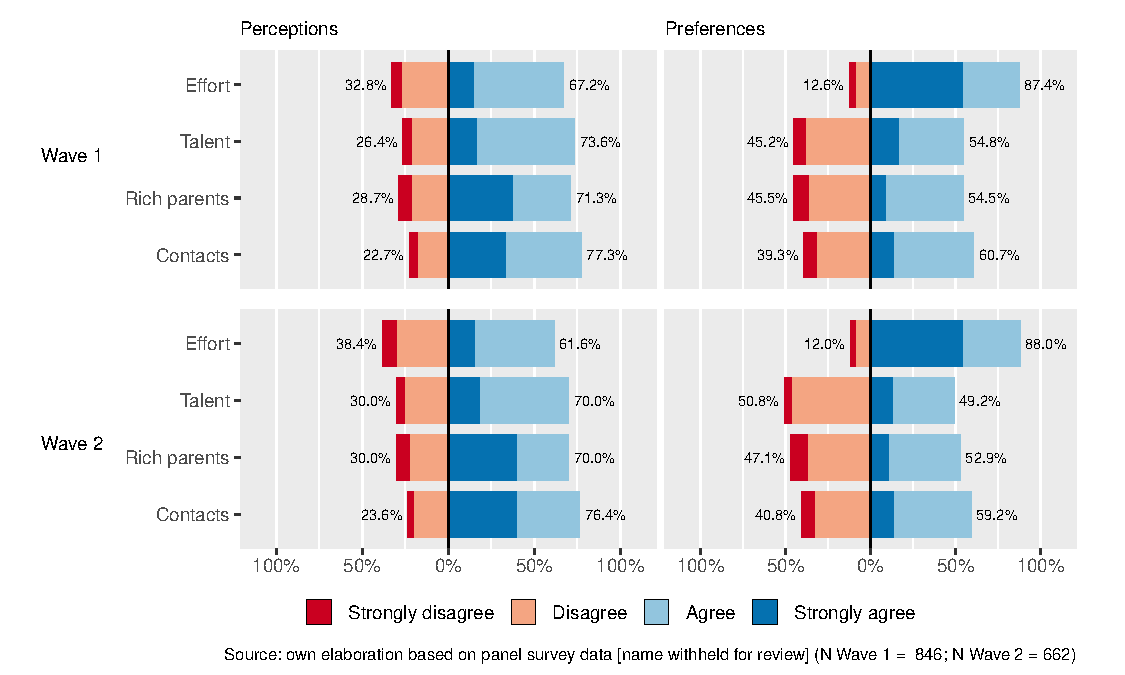
\includegraphics[width=1\linewidth,height=\textheight,keepaspectratio]{paper_BJSE_manuscript_anonymous_files/figure-pdf/fig-likerplot1-1.pdf}

}

\end{figure}%

Figure~\ref{fig-likerplot2} shows the same items by cohort, which
reveals a sharper contrast between perceptions and preferences.
Meritocratic perceptions (effort and talent) receive more agreement in
the primary than in the secondary cohort, while the reverse holds for
privilege perceptions (contacts and family wealth), consistent with a
``disillusionment'' with meritocracy as students progress through school
(\citeproc{ref-fan_disillusionment_2026}{Fan et al., 2026};
\citeproc{ref-tang_meritocratic_2025}{Tang et al., 2025}). Preferences
are more stable across cohorts: effort is the most endorsed basis for
reward, while talent, family wealth, and especially contacts remain more
ambivalent, with contacts more often accepted than rejected in both
cohorts. Overall, the cohort comparison reveals a widening gap between
an effort-centered meritocratic ideal and the perceived importance of
privilege in practice.

\begin{figure}[H]

\caption{\label{fig-likerplot2}Distribution of responses on the scale of
perceptions and preferences regarding meritocracy by cohort}

\centering{

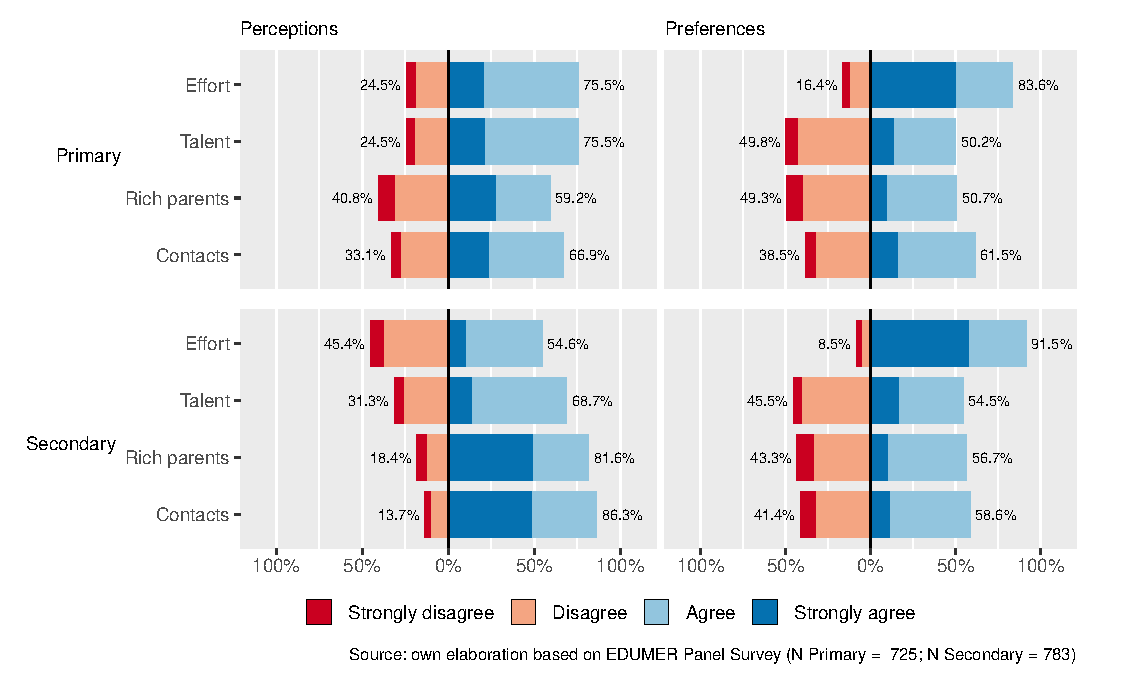
\includegraphics[width=1\linewidth,height=\textheight,keepaspectratio]{paper_BJSE_manuscript_anonymous_files/figure-pdf/fig-likerplot2-1.pdf}

}

\end{figure}%

\subsection{Multidimensional measurement of meritocracy and
privilege}\label{multidimensional-measurement-of-meritocracy-and-privilege}

Figure~\ref{fig-general} presents the measurement model for the pooled
sample (both waves and cohorts), with the four latent dimensions
(circles) each measured by two observed indicators (rectangles). Fit is
reasonable but not fully satisfactory (CFI = 0.97; TLI = 0.94; RMSEA =
0.07): the CFI falls within commonly accepted ranges, but the TLI and
RMSEA do not meet conventional thresholds. Part of this misfit relates
to differences across cohorts, examined in the multigroup analyses
below.

\begin{figure}[H]

\caption{\label{fig-general}Measurement model diagram (pooled sample)}

\centering{

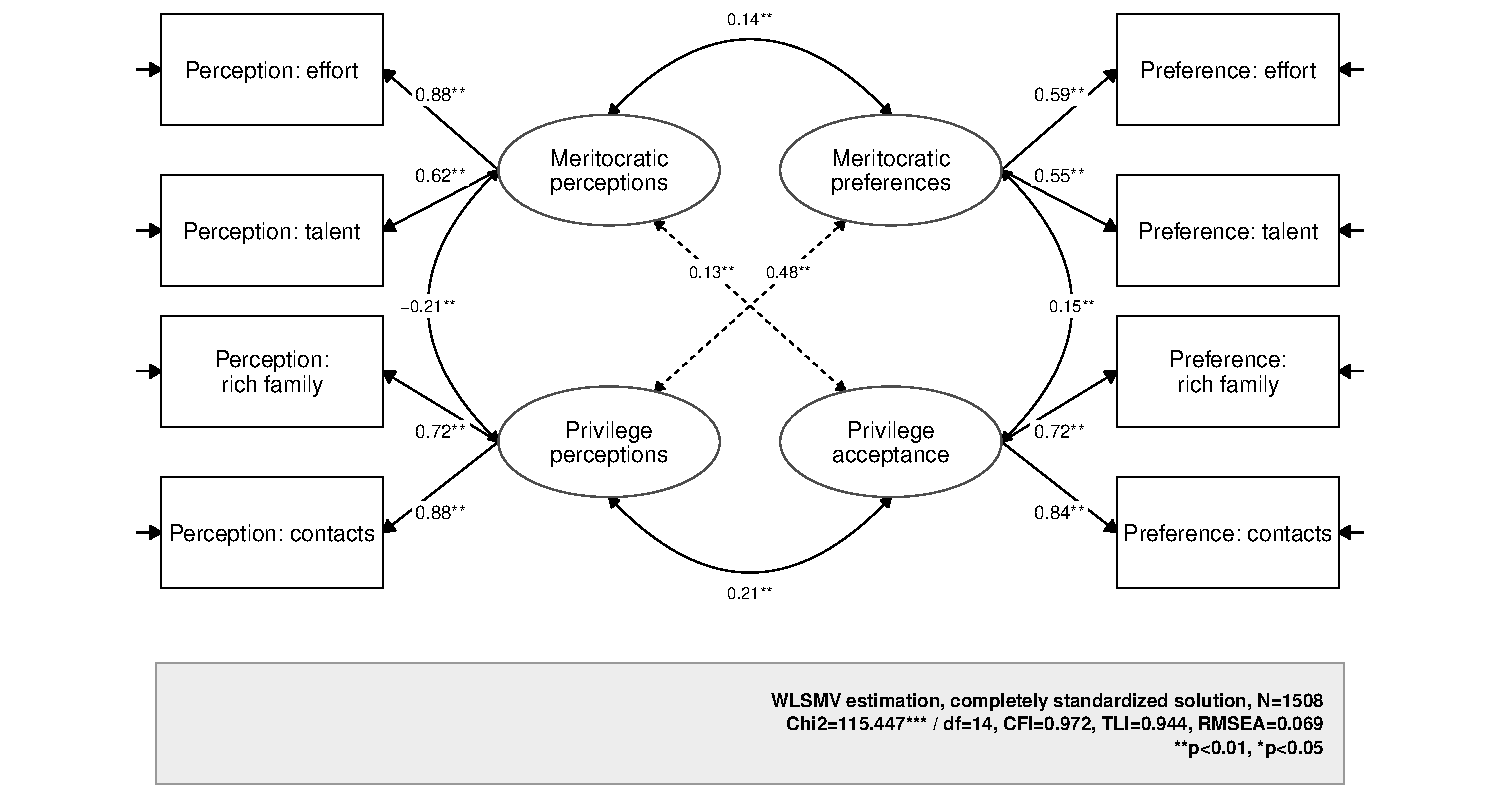
\includegraphics[width=1\linewidth,height=\textheight,keepaspectratio]{paper_BJSE_manuscript_anonymous_files/figure-pdf/fig-general-1.pdf}

}

\end{figure}%

All standardized factor loadings are statistically significant and
moderate to strong: effort (\(\beta\) = 0.88) and talent (\(\beta\) =
0.62) for meritocratic perceptions; effort (\(\beta\) = 0.59) and talent
(\(\beta\) = 0.55) for meritocratic preferences, the weakest pair;
contacts (\(\beta\) = 0.88) and rich family (\(\beta\) = 0.72) for
perceived privilege; and contacts (\(\beta\) = 0.84) and rich family
(\(\beta\) = 0.72) for privilege acceptance. Overall, the indicators are
reasonably good measures of their respective latent constructs.

The latent correlations address \(H_2\). Allowing the four dimensions to
correlate opens the black box of beliefs that both common sense and the
literature often treat as opposite poles of a single continuum. The
dimensions are interrelated but far from perfectly aligned, and all
correlations but one are positive. The only negative correlation is
between meritocratic and privilege perceptions (\(r\) = −0.21):
perceiving society as more meritocratic goes with a lower recognition of
the role of privilege. As among adults
(\citeproc{ref-castillo_multidimensional_2023}{Castillo et al., 2023}),
meritocratic perceptions and preferences are positively correlated
(\(r\) = 0.14). The strongest association is between privilege
perceptions and meritocratic preferences (\(r\) = 0.48): students who
recognize the role of privilege in society are more likely to endorse
meritocratic ideals. Less intuitively, privilege acceptance is
positively correlated with both meritocratic perceptions (\(r\) = 0.13)
and meritocratic preferences (\(r\) = 0.15). Although modest, these last
correlations indicate that merit and privilege beliefs are not simply
opposites but can coexist in students' minds without undermining one
another.

\subsection{Stability of meritocracy and privilege
beliefs}\label{stability-of-meritocracy-and-privilege-beliefs}

\subsubsection{Longitudinal invariance}\label{longitudinal-invariance}

Table~\ref{tbl-longinv} reports the longitudinal invariance tests, in
which the same students measured at two time points are treated as
groups and the unique variances of each item are correlated across waves
(\citeproc{ref-widaman_factorial_2010}{Widaman et al., 2010}). The scale
achieved the strongest level, strict invariance: the strict model fit
well, \(\chi^2\)(84) = 130.17, CFI = 0.991, RMSEA = 0.031 (90\% CI:
0.020--0.040), and its fit was practically identical to that of the
strong model, \(\Delta \chi^2\)(4) = 1.635, \(\Delta\)CFI = 0.000,
\(\Delta\)RMSEA = −0.002, well within commonly used cutoffs
(\citeproc{ref-chen_sensitivity_2007}{Chen, 2007}).

\begin{table}[H]

\caption{\label{tbl-longinv}Longitudinal invariance results}

\centering{

\centering\begingroup\fontsize{9.5}{11.5}\selectfont

\resizebox{\ifdim\width>\linewidth\linewidth\else\width\fi}{!}{
\begin{tabular}{>{\centering\arraybackslash}p{2cm}>{\centering\arraybackslash}p{2.1cm}>{\centering\arraybackslash}p{1.3cm}>{\centering\arraybackslash}p{2.2cm}>{\centering\arraybackslash}p{2.4cm}>{\centering\arraybackslash}p{1.3cm}>{\centering\arraybackslash}p{1.4cm}>{\centering\arraybackslash}p{2cm}}
\toprule
Model & $\chi^2$ (df) & CFI & RMSEA (90\% CI) & $\Delta \chi^2$ ($\Delta$df) & $\Delta$CFI & $\Delta$RMSEA & Decision\\
\midrule
Configural & 117.7 (68) & 0.991 & 0.035 
 (0.024-0.046) & 0 (0) & 0 & 0.000 & Reference\\
Weak & 122.51 (72) & 0.990 & 0.034 
 (0.024-0.045) & 4.809 (4) & 0 & -0.001 & Accept\\
Strong & 128.53 (80) & 0.991 & 0.032 
 (0.021-0.042) & 6.02 (8) & 0 & -0.002 & Accept\\
Strict & 130.17 (84) & 0.991 & 0.031 
 (0.02-0.04) & 1.635 (4) & 0 & -0.002 & Accept\\
\bottomrule
\end{tabular}}
\endgroup{}

}

\end{table}%

Longitudinal invariance implies that changes in students' scores can be
interpreted as true changes in their beliefs rather than artifacts of
measurement. Table~\ref{tbl-latmeans} reports the latent means from the
strict model, with wave 1 means fixed to zero, so that the wave 2
estimates are the between-wave changes, tested with Wald tests. Latent
means are in the metric of each factor's first indicator, and \(d\)
expresses the change in wave 1 latent standard deviations. No dimension
changed significantly between waves (all adjusted \(p\) \textgreater{}
.30). Perceived meritocracy declined slightly (\(\Delta\) = −0.29, \(p\)
= .118, \(d\) = −0.14) and perceived privilege increased slightly
(\(\Delta\) = 0.15, \(p\) = .080, \(d\) = 0.13), a direction compatible
with a growing perception of privilege, but neither difference is
reliably different from zero. Preferences were practically unchanged,
both for meritocracy (\(\Delta\) = −0.08, \(p\) = .458) and for the
acceptance of privilege (\(\Delta\) = −0.12, \(p\) = .119). Overall,
students' beliefs were stable over the period.

\begin{table}[H]

\caption{\label{tbl-latmeans}Latent means of meritocracy and privilege
dimensions by wave}

\centering{

\centering\begingroup\fontsize{9.5}{11.5}\selectfont

\resizebox{\ifdim\width>\linewidth\linewidth\else\width\fi}{!}{
\begin{tabular}{>{\raggedright\arraybackslash}p{5.5cm}cccccc}
\toprule
Dimension & Wave 1 & Wave 2 (SE) & $z$ & $p$ & $p$ (Holm) & $d$\\
\midrule
Perceived meritocracy (effort and talent) & 0 (ref.) & -0.286 (0.183) & -1.56 & .118 & .354 & -0.14\\
Perceived privilege (rich parents and contacts) & 0 (ref.) & 0.149 (0.085) & 1.75 & .080 & .320 & 0.13\\
Preference for meritocracy (effort and talent) & 0 (ref.) & -0.075 (0.101) & -0.74 & .458 & .458 & -0.08\\
Acceptance of privilege (rich parents and contacts) & 0 (ref.) & -0.115 (0.074) & -1.56 & .119 & .354 & -0.10\\
\bottomrule
\end{tabular}}
\endgroup{}

}

\end{table}%

\vspace{-1.2em}\footnotesize \emph{Note:} Latent means from the strict
longitudinal invariance model (\(N\) = 591); wave 1 means are fixed to 0
(reference). Wave 2 estimates are the wave 2 − wave 1 differences,
tested with Wald tests; \(p\) (Holm) adjusts for the four comparisons.
\(d\) = difference divided by the latent standard deviation in wave 1.
\par\normalsize

\subsection{Cohorts comparability}\label{cohorts-comparability}

Table~\ref{tbl-cohortinv} reports the cross-cohort (multigroup)
invariance tests comparing primary and secondary students, using wave 1
data. The configural model, which imposes the same four-factor structure
in both cohorts, fits well, \(\chi^2\)(28) = 47.65, CFI = 0.991, RMSEA =
0.041. Weak invariance, however, was not achieved: constraining the
factor loadings to be equal significantly worsened fit,
\(\Delta \chi^2\)(4) = 20.77, \(p\) \textless{} .001, although the
changes in CFI (\(\Delta\)CFI = −0.009) and RMSEA (\(\Delta\)RMSEA =
0.013) remain just within conventional cutoffs
(\citeproc{ref-chen_sensitivity_2007}{Chen, 2007}), so at the global
level the evidence against loading invariance is not overwhelming.
Adding equality constraints on the thresholds, which play the role of
intercepts for ordinal items, worsened fit further, \(\Delta \chi^2\)(8)
= 35.89, \(p\) \textless{} .001, with \(\Delta\)CFI = −0.011, which
exceeds the recommended cutoff. The alternative sequence proposed by
Svetina et al. (\citeproc{ref-svetina_multiplegroup_2020}{2020}), which
tests thresholds before loadings, led to the same conclusion (see
supplementary material). The relationship between the latent factors and
their indicators therefore differs between primary and secondary
students, which could reflect developmental differences or differences
in how the items are interpreted.

\begin{table}[H]

\caption{\label{tbl-cohortinv}Cohort (multigroup) invariance results}

\centering{

\centering\begingroup\fontsize{9.5}{11.5}\selectfont

\resizebox{\ifdim\width>\linewidth\linewidth\else\width\fi}{!}{
\begin{tabular}{>{\centering\arraybackslash}p{3.6cm}>{\centering\arraybackslash}p{2.1cm}>{\centering\arraybackslash}p{1.3cm}>{\centering\arraybackslash}p{2.2cm}>{\centering\arraybackslash}p{2.4cm}>{\centering\arraybackslash}p{1.3cm}>{\centering\arraybackslash}p{1.4cm}>{\centering\arraybackslash}p{2cm}}
\toprule
Model & $\chi^2$ (df) & CFI & RMSEA (90\% CI) & $\Delta \chi^2$ ($\Delta$df) & $\Delta$CFI & $\Delta$RMSEA & Decision\\
\midrule
\addlinespace[0.3em]
\multicolumn{8}{l}{\textbf{Full invariance sequence}}\\
\hspace{1em}Configural & 47.65 (28) & 0.991 & 0.041 (0.019-0.06) &  &  &  & Reference\\
\hspace{1em}Loadings & 71.3 (32) & 0.981 & 0.054 (0.037-0.071) & 20.77 (4) *** & -0.009 & 0.013 & Reject\\
\hspace{1em}Loadings + Thresholds & 103.09 (40) & 0.970 & 0.061 (0.047-0.076) & 35.89 (8) *** & -0.011 & 0.007 & Reject\\
\addlinespace[0.3em]
\multicolumn{8}{l}{\textbf{Partial invariance (loading of preferences for talent freed)}}\\
\hspace{1em}Loadings (partial) & 48.48 (31) & 0.992 & 0.037 (0.014-0.056) & 1.82 (3) & 0.001 & -0.004 & Accept\\
\hspace{1em}Loadings (partial) + Thresholds & 84.91 (39) & 0.978 & 0.053 (0.037-0.068) & 42.72 (8) *** & -0.014 & 0.016 & Reject\\
\bottomrule
\end{tabular}}
\endgroup{}

\begingroup\fontsize{8}{9.5}\selectfont

\raggedright

\textit{Note.} Scaled WLSMV statistics. Each model is compared with the
preceding one in its block (partial loadings: vs.~configural).

\par\endgroup

}

\end{table}%

To identify the source of non-invariance, we inspected univariate score
tests for each equality constraint on the loadings. The misfit was
concentrated in a single parameter: the loading of the talent preference
item on the meritocratic preferences factor (\(\chi^2\)(1) = 16.87,
Holm-adjusted \(p\) \textless{} .001). The remaining loadings were fully
consistent with invariance (all \(p\) \textgreater{} .36). Accordingly,
freeing that single loading is enough to restore weak invariance, with a
fit indistinguishable from the configural model, \(\Delta \chi^2\)(3) =
1.82, \(p\) = .61, CFI = 0.992, RMSEA = 0.037.

The cohort-specific loadings (see supplementary material) show what this
means substantively. In primary school the meritocratic preferences
factor is defined mainly by the preference for talent as a criterion of
reward (standardized loading = 0.87) and much less by the preference for
effort (0.45). In secondary school the pattern reverses: effort becomes
the core of the factor (0.83) whereas talent is only weakly related to
it (0.37). The meritocratic preferences factor thus does not carry an
equivalent meaning across cohorts, which may reflect a change in how
students interpret meritocratic principles over the school years, and
its levels should be compared across cohorts with caution. In contrast,
the loadings of the other three factors are equivalent across cohorts.

Even after freeing this loading, adding the threshold constraints
significantly worsened fit (\(\Delta \chi^2\)(8) = 42.72, \(p\)
\textless{} .001; \(\Delta\)CFI = −0.014), so strong invariance was also
not achieved. In this case, the source is different: univariate score
tests point to the thresholds of the perceived effort item, for which
all three constraints are violated (\(\chi^2\)(1) between 11.6 and 11.9;
Holm-adjusted \(p\) between .015 and .017), whereas no threshold of any
other item shows meaningful misfit (adjusted \(p\) \textgreater{} .99).
Substantively, students in the two cohorts use the response categories
of this item differently for a given level of perceived meritocracy,
which is consistent with the differences reported in the descriptive
section (see Figure~\ref{fig-likerplot2}): secondary students are more
likely to endorse the lowest response category when judging whether
effort is rewarded in society, suggesting that they apply different
criteria. Taken together, only partial weak invariance holds, and
comparisons of latent means across cohorts, in particular for
meritocratic perceptions, should be interpreted with caution.

\section{Discussion}\label{discussion}

Meritocracy and privilege are often treated as opposite poles of a
single continuum, but the present study shows that they are better
understood as distinct dimensions that coexist in students' minds, as
found among adults
(\citeproc{ref-castillo_multidimensional_2023}{Castillo et al., 2023}).
As expected in \(H_1\), the four latent constructs (perceived
meritocracy, perceived privilege, meritocratic preferences, and
privilege acceptance) are identifiable in the school-aged population,
with satisfactory model fit and strong factor loadings in the two waves
analyzed. Even at an early stage of school socialization, students
distinguish between meritocratic and privilege-based perceptions and
preferences. This structure resonates with qualitative evidence from
Chilean schools, where students across socioeconomic groups
simultaneously invoke meritocratic ideals and recognize structural
advantage (\citeproc{ref-neutaguayo_neoliberalism_2025}{Neut Aguayo et
al., 2025}), and where merit is often defined by attitude and visible
effort rather than by academic outcomes
(\citeproc{ref-moyanodavila_merit_2025}{Moyano Dávila et al., 2025}).
Where merit is primarily understood as a behavioral disposition,
accepting that privilege leads to better outcomes may not be experienced
as a contradiction but as a separate normative judgment, which suggests
that the coexistence of these orientations reflects how students
navigate competing narratives about fairness and reward, rather than an
artifact of survey design.

The empirical separability of these dimensions, and the associations
among them (\(H_2\)), have implications for how meritocratic beliefs are
understood and measured
(\citeproc{ref-kwon_multidimensionality_2024}{Kwon \& Pandian, 2024};
\citeproc{ref-mijs_visualizing_2026}{Mijs, 2026};
\citeproc{ref-zhu_meritocratic_2025}{Zhu, 2025}). First, perceived
privilege is positively associated with stronger meritocratic
preferences, consistent with a normative-reactive response to perceived
unfairness (\citeproc{ref-castillo_multidimensional_2023}{Castillo et
al., 2023}). Second, meritocratic perceptions are positively correlated
with privilege acceptance. Prior research has linked meritocratic
perceptions to the self-interest hypothesis, whereby those in higher
social positions are more likely to adopt a meritocratic worldview
(\citeproc{ref-heuer_legitimizing_2020}{Heuer et al., 2020}).
Incorporating privilege reveals a more complex picture: perceiving
society as meritocratic may also conceal support for privilege, so that
the justification of inequality is embedded in the meritocratic
narrative itself (\citeproc{ref-khan_saying_2013}{Khan \& Jerolmack,
2013}). These results are consistent with Zhu's
(\citeproc{ref-zhu_meritocratic_2025}{2025}) argument that meritocratic
and structural explanations accumulate rather than displace one another,
with accounts in which merit endorsement remains stable as recognition
of structural constraints increases (\citeproc{ref-liu_does_2025}{C. Liu
\& Wang, 2025}; \citeproc{ref-tang_meritocratic_2025}{Tang et al.,
2025}), and with the distinct attitudinal clusters in which Kwon \&
Pandian (\citeproc{ref-kwon_multidimensionality_2024}{2024}) show that
coexistence takes different forms across individuals.

These results also bear on how the literature on school meritocracy
should be read. Research has linked stronger meritocratic beliefs among
students to inequality legitimation, weaker support for redistribution,
and greater acceptance of unequal access to educational resources
(\citeproc{ref-batruch_belief_2022}{Batruch et al., 2022};
\citeproc{ref-castillo_socialization_2024}{Castillo et al., 2024};
\citeproc{ref-wiederkehr_belief_2015}{Wiederkehr et al., 2015}), but
mostly with unidimensional or undifferentiated measures that cannot
establish whether these effects are specific to particular dimensions.
Our findings suggest that they are likely dimension-specific: perceived
meritocracy is not equivalent to preferred meritocracy, and neither
carries the same consequences as perceived privilege or privilege
acceptance. Chauvin et al. (\citeproc{ref-chauvin_school_2026}{2026})
similarly distinguish ability and equity, but their measure is confined
to perceived meritocracy among teachers. The present study provides a
multidimensional measurement of meritocratic and privilege beliefs
applicable to students, which makes it possible to examine whether
distinct dimensions carry distinct consequences for the educational
environment, from students' sense of justice in school to civic
attitudes and the broader climate of fairness.

Regarding \(H_3\), strict longitudinal invariance indicates that the
scale measures the same constructs across waves, so that changes over
time reflect real within-student change rather than shifts in how items
are interpreted (\citeproc{ref-liu_testing_2017}{Y. Liu et al., 2017};
\citeproc{ref-putnick_measurement_2016}{Putnick \& Bornstein, 2016}).
Meritocratic belief structures appear fairly stable over one year in
early-to-mid adolescence, which gives further studies in this agenda a
sound measurement basis. Invariance across educational levels, however,
was not supported. The non-invariance is concentrated in two parameters:
the relative weight of talent and effort in meritocratic preferences,
and how students read whether effort is rewarded. We do not consider
this finding reducible to a mere measurement failure. Rather, we
interpret it as older students attaching different meanings to these
items, linked to their more sophisticated reasoning about fairness and
to their growing exposure to school sorting such as grades, tracking,
and peer comparison. The declining centrality of talent in older
students' meritocratic preferences may reflect a gradual disenchantment
with inherited attributes, a kind of ``reality shock''
(\citeproc{ref-allen_top_2016}{Allen, 2016};
\citeproc{ref-henry_development_2006}{Henry \& Saul, 2006};
\citeproc{ref-resh_sense_2014}{Resh \& Sabbagh, 2014};
\citeproc{ref-tang_meritocratic_2025}{Tang et al., 2025}). This could be
related to Chile's stratified system, where the gap between meritocratic
discourse and structural reality can be experienced as a moral grievance
(\citeproc{ref-neutaguayo_neoliberalism_2025}{Neut Aguayo et al.,
2025}), but research in other contexts could help shed light on this
issue.

\section{Conclusions}\label{conclusions}

Schools socialize students into beliefs about meritocracy, promoting
effort and talent as the legitimate basis of reward while simultaneously
exposing them to the weight of family resources and social connections
in shaping outcomes (\citeproc{ref-goudeau_hidden_2017a}{Goudeau \&
Croizet, 2017}; \citeproc{ref-resh_sense_2014}{Resh \& Sabbagh, 2014};
\citeproc{ref-traini_stratification_2022}{Traini, 2022}). Students
navigate this tension by holding both orientations at once, endorsing
merit as an ideal while recognizing that privilege structures actual
outcomes, a configuration that can be associated with \emph{dual
consciousness} (\citeproc{ref-kluegel_beliefs_1987}{Kluegel \& Smith,
1987}; \citeproc{ref-liu_does_2025}{C. Liu \& Wang, 2025};
\citeproc{ref-tang_meritocratic_2025}{Tang et al., 2025}). Extending
Castillo et al.'s (\citeproc{ref-castillo_multidimensional_2023}{2023})
multidimensional framework to two cohorts of Chilean students (6th and
9th graders in 2023, followed into 7th and 10th grade in 2024), this
study shows that these beliefs can be measured reliably in school-aged
populations, and equivalently over time. This is a modest but
foundational contribution: a precondition for studying the developmental
trajectory of meritocratic beliefs and their educational implications,
such as gender and social class differences.

Although this study draws on a single country, three of its
contributions are likely to travel across educational systems. First,
the distinctions between perceived and preferred meritocracy, and
between meritocratic and privilege-based principles, reflect cognitive
and normative capacities that develop during adolescence regardless of
national context, although whether the four-factor structure replicates
in other societies remains to be established. Second, the coexistence of
merit endorsement and recognition of privilege has been documented in
China (\citeproc{ref-liu_does_2025}{C. Liu \& Wang, 2025};
\citeproc{ref-tang_meritocratic_2025}{Tang et al., 2025}), the United
States and Finland (\citeproc{ref-zhu_meritocratic_2025}{Zhu, 2025}),
and Europe (\citeproc{ref-kwon_multidimensionality_2024}{Kwon \&
Pandian, 2024}), suggesting it is not a Chilean peculiarity. Third,
longitudinal invariance testing as a prerequisite for developmental
inference applies to any panel study of meritocratic beliefs. By
contrast, the cross-cohort non-invariance may be more system-dependent,
reflecting the intensity and timing of school-based sorting in Chile's
tracked and marketized system
(\citeproc{ref-madariaga_three_2020}{Madariaga, 2020};
\citeproc{ref-valenzuela_socioeconomic_2013}{Valenzuela et al., 2013});
research in countries with different tracking regimes will help clarify
which aspects of measurement equivalence are universal.

This study has limitations that also point to directions for future
research. First, the scale relies on two items per factor, which
restricts both content coverage and reliability. Second, the design
comprises only two waves and two school levels; additional waves and a
broader age range are needed to trace developmental trajectories and to
establish when the meaning students attach to meritocracy begins to
shift. Third, and most consequentially, the lack of invariance across
school cohorts indicates that meritocracy scales cannot be assumed to
function equivalently across educational stages. Future studies should
therefore examine differential item functioning, develop stage-sensitive
item formulations, and adopt partial-invariance approaches
(\citeproc{ref-putnick_measurement_2016}{Putnick \& Bornstein, 2016};
\citeproc{ref-vandeschoot_checklist_2012}{Van De Schoot et al., 2012}).
This would allow a more rigorous examination of group differences, such
as the gender differences in meritocratic beliefs suggested by Gogescu
(\citeproc{ref-gogescu_meritocracy_2025}{2025}) and Khan \& Jerolmack
(\citeproc{ref-khan_saying_2013}{2013}), and of how beliefs about merit
and privilege relate to the school outcomes for which they are likely to
matter most: students' sense of justice and fairness, civic attitudes
and engagement, perceptions of school climate, wellbeing, and academic
motivation.

\textbf{Data availability statement}: The data and code that support the
findings of this study are available in a GitHub repository. To preserve
anonymity during peer review, the repository address is not included in
this version of the manuscript; it can be provided to the editor upon
request. Upon publication, the data and code will be deposited in a
permanent public repository with a persistent identifier.

\textbf{Disclosure statement}: The authors report there are no competing
interests to declare.

\textbf{Declaration of Generative AI Use}: Generative AI was used for
manuscript proofreading and for supporting the formatting of graphs and
tables. For these tasks, we used Claude Sonnet 5.5 (Anthropic). The
authors reviewed all AI-assisted output and take full responsibility for
the content of the manuscript.

\section{References}\label{references}

\phantomsection\label{refs}
\begin{CSLReferences}{1}{0}
\bibitem[\citeproctext]{ref-allen_top_2016}
Allen, K. (2016). Top girls navigating austere times: Interrogating
youth transitions since the {``crisis.''} \emph{Journal of Youth
Studies}, \emph{19}(6), 805--820.
\url{https://doi.org/10.1080/13676261.2015.1112885}

\bibitem[\citeproctext]{ref-batruch_belief_2022}
Batruch, A., Jetten, J., Van de Werfhorst, H., Darnon, C., \& Butera, F.
(2022). Belief in school meritocracy and the legitimization of social
and income inequality. \emph{Social Psychological and Personality
Science}, 194855062211110.
\url{https://doi.org/10.1177/19485506221111017}

\bibitem[\citeproctext]{ref-bernstein_pedagogy_1996}
Bernstein, B. B. (1996). \emph{Pedagogy, symbolic control, and identity
: Theory, research, critique}. London ; Washington, D.C. : Taylor \&
Francis. Retrieved from
\url{http://archive.org/details/pedagogysymbolic0000bern}

\bibitem[\citeproctext]{ref-bourdieu_reproduction_1990}
Bourdieu, P., \& Passeron, J. C. (1990). \emph{Reproduction in
education, society and culture} (Second Edition). Sage Publications Ltd.

\bibitem[\citeproctext]{ref-brown_confirmatory_2015}
Brown, T. A. (2015). \emph{Confirmatory factor analysis for applied
research} (Second edition). New York London: The Guilford Press.

\bibitem[\citeproctext]{ref-busemeyer_skills_2014}
Busemeyer, M. (2014). \emph{Skills and inequality: Partisan politics and
the political economy of education reforms in western welfare states}.
Cambridge University Press.

\bibitem[\citeproctext]{ref-castillo_multidimensional_2023}
Castillo, J. C., Iturra, J., Maldonado, L., Atria, J., \& Meneses, F.
(2023). A multidimensional approach for measuring meritocratic beliefs:
Advantages, limitations and alternatives to the ISSP social inequality
survey. \emph{International Journal of Sociology}, \emph{53}(6),
448--472. \url{https://doi.org/10.1080/00207659.2023.2274712}

\bibitem[\citeproctext]{ref-castillo_socialization_2024}
Castillo, J. C., Salgado, M., Carrasco, K., \& Laffert, A. (2024). The
socialization of meritocracy and market justice preferences at school.
\emph{Societies}, \emph{14}(11), 214.
\url{https://doi.org/10.3390/soc14110214}

\bibitem[\citeproctext]{ref-chauvin_school_2026}
Chauvin, B., Rauscher, C., Saidah, B., \& Louvet, E. (2026). School
meritocracy: A multidimensional construct? Evidence from the development
of a school meritocracy scale by exploratory and confirmatory bifactor
modeling. \emph{Current Psychology}, \emph{45}(5), 519.
\url{https://doi.org/10.1007/s12144-026-09134-1}

\bibitem[\citeproctext]{ref-chen_sensitivity_2007}
Chen, F. F. (2007). Sensitivity of goodness of fit indexes to lack of
measurement invariance. \emph{Structural Equation Modeling: A
Multidisciplinary Journal}, \emph{14}(3), 464--504.
\url{https://doi.org/10.1080/10705510701301834}

\bibitem[\citeproctext]{ref-darnon_where_2018}
Darnon, C., Wiederkehr, V., Dompnier, B., \& Martinot, D. (2018).
{``Where there is a will, there is a way''}: Belief in school
meritocracy and the social-class achievement gap. \emph{British Journal
of Social Psychology}, \emph{57}(1), 250--262.
\url{https://doi.org/10.1111/bjso.12214}

\bibitem[\citeproctext]{ref-davey_preference_1999}
Davey, L. M., Bobocel, D. R., Son Hing, L. S., \& Zanna, M. P. (1999).
Preference for the merit principle scale: An individual difference
measure of distributive justice preferences. \emph{Social Justice
Research}, \emph{12}(3), 223--240.
\url{https://doi.org/10.1023/A:1022148418210}

\bibitem[\citeproctext]{ref-davidov_measurement_2014}
Davidov, E., Meuleman, B., Cieciuch, J., Schmidt, P., \& Billiet, J.
(2014). Measurement equivalence in cross-national research. \emph{Annual
Review of Sociology}, \emph{40}(Volume 40, 2014), 55--75.
\url{https://doi.org/10.1146/annurev-soc-071913-043137}

\bibitem[\citeproctext]{ref-deng_its_2025}
Deng, Y., \& Wang, F. (2025). It's my fault, i should try harder! The
narratives of self‐made upward mobility sustain belief in meritocracy in
low social mobility context. \emph{British Journal of Psychology},
bjop.70015. \url{https://doi.org/10.1111/bjop.70015}

\bibitem[\citeproctext]{ref-duru-bellat_whos_2012}
Duru-Bellat, M., \& Tenret, E. (2012). Who's for meritocracy? Individual
and contextual variations in the faith. \emph{Comparative Education
Review}, \emph{56}(2), 223--247. \url{https://doi.org/10.1086/661290}

\bibitem[\citeproctext]{ref-fan_disillusionment_2026}
Fan, S., John, O. P., \& De Fruyt, F. (2026). Disillusionment with
meritocracy during the transition to adulthood: Longitudinal change in
belief systems and depression in china. \emph{Psychological Science},
09567976261479675. \url{https://doi.org/10.1177/09567976261479675}

\bibitem[\citeproctext]{ref-ferre_welfare_2023}
Ferre, J. C. (2023). Welfare regimes in twenty-first-century latin
america. \emph{Journal of International and Comparative Social Policy},
\emph{39}(2), 101--127. \url{https://doi.org/10.1017/ics.2023.16}

\bibitem[\citeproctext]{ref-garcia-sierra_dark_2023}
García-Sierra, A. (2023). The dark side of meritocratic beliefs: Is
believing in meritocracy detrimental to individuals from low
socioeconomic backgrounds? \emph{Social Justice Research}, \emph{36}(4),
385--409. \url{https://doi.org/10.1007/s11211-023-00413-x}

\bibitem[\citeproctext]{ref-gingrich_making_2011}
Gingrich, J. R. (2011). \emph{Making markets in the welfare state: The
politics of varying market reforms} (1st ed.). Cambridge University
Press. \url{https://doi.org/10.1017/CBO9780511791529}

\bibitem[\citeproctext]{ref-gogescu_meritocracy_2025}
Gogescu, F. (2025). Meritocracy seen through the eyes of its champions:
A comparative study of educational elites. \emph{British Journal of
Sociology of Education}, \emph{46}(1), 34--53.
\url{https://doi.org/10.1080/01425692.2024.2418097}

\bibitem[\citeproctext]{ref-goudeau_hidden_2017a}
Goudeau, S., \& Croizet, J.-C. (2017). Hidden advantages and
disadvantages of social class: How classroom settings reproduce social
inequality by staging unfair comparison. \emph{Psychological Science},
\emph{28}(2), 162--170. \url{https://doi.org/10.1177/0956797616676600}

\bibitem[\citeproctext]{ref-henry_development_2006}
Henry, P. J., \& Saul, A. (2006). The development of system
justification in the developing world. \emph{Social Justice Research},
\emph{19}(3), 365--378. \url{https://doi.org/10.1007/s11211-006-0012-x}

\bibitem[\citeproctext]{ref-heuer_legitimizing_2020}
Heuer, J.-O., Lux, T., Mau, S., \& Zimmermann, K. (2020). Legitimizing
inequality: The moral repertoires of meritocracy in four countries.
\emph{Comparative Sociology}, \emph{19}(4-5), 542--584.
\url{https://doi.org/10.1163/15691330-BJA10017}

\bibitem[\citeproctext]{ref-imhoff_nociones_2025}
Imhoff, D., \& Brussino, S. (2025). Nociones infantiles sobre
desigualdad social: atravesamientos ideológicos y procesos de
socialización política. \emph{Revista Latinoamericana de Ciencias
Sociales, Niñez y Juventud}, \emph{13}(2).
\url{https://doi.org/10.11600/1692715x.1329071114}

\bibitem[\citeproctext]{ref-jost_decade_2004a}
Jost, J. T., Banaji, M. R., \& Nosek, B. A. (2004). A decade of system
justification theory: Accumulated evidence of conscious and unconscious
bolstering of the status quo. \emph{Political Psychology}, \emph{25}(6),
881--919. \url{https://doi.org/10.1111/j.1467-9221.2004.00402.x}

\bibitem[\citeproctext]{ref-khan_privilege_2013}
Khan, S. (2013). \emph{Privilege: The making of an adolescent elite at
st. Paul's school} (4. printing, and first paperback printing).
Princeton, N.J. Woodstock: Princeton University Press.

\bibitem[\citeproctext]{ref-khan_saying_2013}
Khan, S., \& Jerolmack, C. (2013). Saying meritocracy and doing
privilege. \emph{The Sociological Quarterly}, \emph{54}(1), 9--19.
\url{https://doi.org/10.1111/tsq.12008}

\bibitem[\citeproctext]{ref-kline_principles_2023}
Kline, R. B. (2023). \emph{Principles and practice of structural
equation modeling}. Guilford Publications.

\bibitem[\citeproctext]{ref-kluegel_beliefs_1987}
Kluegel, J. R., \& Smith, E. R. (1987). \emph{Beliefs about inequality:
Americans' views of what is and what ought to be}. New York: Routledge.

\bibitem[\citeproctext]{ref-krosnick_aging_1989}
Krosnick, J. A., \& Alwin, D. F. (1989). Aging and susceptibility to
attitude change. \emph{Journal of Personality and Social Psychology},
\emph{57}(3), 416--425. \url{https://doi.org/10.1037/0022-3514.57.3.416}

\bibitem[\citeproctext]{ref-kwon_multidimensionality_2024}
Kwon, R., \& Pandian, R. K. (2024). Multidimensionality in merit
attitudes: The role of hard work, skills, and social connections in
europe. \emph{Social Science Research}, \emph{122}, 103056.
\url{https://doi.org/10.1016/j.ssresearch.2024.103056}

\bibitem[\citeproctext]{ref-lareau_unequal_2003}
Lareau, A. (2003). \emph{Unequal childhoods: Class, race, and family
life}. Berkeley: University of California Press.

\bibitem[\citeproctext]{ref-leitgob_measurement_2023}
Leitgöb, H., Seddig, D., Asparouhov, T., Behr, D., Davidov, E., De
Roover, K., \ldots{} van de Schoot, R. (2023). Measurement invariance in
the social sciences: Historical development, methodological challenges,
state of the art, and future perspectives. \emph{Social Science
Research}, \emph{110}, 102805.
\url{https://doi.org/10.1016/j.ssresearch.2022.102805}

\bibitem[\citeproctext]{ref-liu_does_2025}
Liu, C., \& Wang, J. (2025). Does education legitimise inequality?
Comparative analysis of income inequality, education, and meritocratic
beliefs. \emph{The British Journal of Sociology}, 1468--4446.70029.
\url{https://doi.org/10.1111/1468-4446.70029}

\bibitem[\citeproctext]{ref-liu_testing_2017}
Liu, Y., Millsap, R. E., West, S. G., Tein, J.-Y., Tanaka, R., \& Grimm,
K. J. (2017). Testing measurement invariance in longitudinal data with
ordered-categorical measures. \emph{Psychological Methods},
\emph{22}(3), 486--506. \url{https://doi.org/10.1037/met0000075}

\bibitem[\citeproctext]{ref-lundberg_what_2021}
Lundberg, I., Johnson, R., \& Stewart, B. M. (2021). What is your
estimand? Defining the target quantity connects statistical evidence to
theory. \emph{American Sociological Review}, \emph{86}(3), 532--565.
\url{https://doi.org/10.1177/00031224211004187}

\bibitem[\citeproctext]{ref-madariaga_three_2020}
Madariaga, A. (2020). The three pillars of neoliberalism: Chile's
economic policy trajectory in comparative perspective.
\emph{Contemporary Politics}, \emph{26}(3), 308--329.
\url{https://doi.org/10.1080/13569775.2020.1735021}

\bibitem[\citeproctext]{ref-mijs_unfulfillable_2016}
Mijs, J. (2016). The unfulfillable promise of meritocracy: Three lessons
and their implications for justice in education. \emph{Social Justice
Research}, \emph{29}(1), 14--34.
\url{https://doi.org/10.1007/s11211-014-0228-0}

\bibitem[\citeproctext]{ref-mijs_paradox_2021}
Mijs, J. (2021). The paradox of inequality: Income inequality and belief
in meritocracy go hand in hand. \emph{Socio-Economic Review},
\emph{19}(1), 7--35. \url{https://doi.org/10.1093/ser/mwy051}

\bibitem[\citeproctext]{ref-mijs_visualizing_2026}
Mijs, J. (2026). Visualizing belief in merit and privilege, 1930 to
2020: rejoinder. \emph{Socius: Sociological Research for a Dynamic
World}, \emph{12}, 23780231261426413.
\url{https://doi.org/10.1177/23780231261426413}

\bibitem[\citeproctext]{ref-moyanodavila_merit_2025}
Moyano Dávila, C., Alarcón-Arcos, S., Angelcos, N., Castillo, J. C., \&
Salgado, M. (2025). Merit as an attitude: Chilean school communities'
repertoires in chile and the perception of the {``good student''} in a
post-pandemic scenario. \emph{Social Justice Research}, \emph{38}(3),
264--289. \url{https://doi.org/10.1007/s11211-025-00456-2}

\bibitem[\citeproctext]{ref-neutaguayo_neoliberalism_2025}
Neut Aguayo, P., Rivera-Vargas, P., \& Miño Puigcercós, R. (2025).
Neoliberalism and school inequality in the chilean education system: An
analysis from the voices of lower-class, middle-class, and upper-class
students. \emph{International Studies in Sociology of Education}, 1--16.
\url{https://doi.org/10.1080/09620214.2025.2558938}

\bibitem[\citeproctext]{ref-putnick_measurement_2016}
Putnick, D. L., \& Bornstein, M. H. (2016). Measurement invariance
conventions and reporting: The state of the art and future directions
for psychological research. \emph{Developmental Review}, \emph{41},
71--90. \url{https://doi.org/10.1016/j.dr.2016.06.004}

\bibitem[\citeproctext]{ref-resh_sense_2014}
Resh, N., \& Sabbagh, C. (2014). Sense of justice in school and civic
attitudes. \emph{Social Psychology of Education}, \emph{17}(1), 51--72.
\url{https://doi.org/10.1007/s11218-013-9240-8}

\bibitem[\citeproctext]{ref-reynolds_perceptions_2014}
Reynolds, J., \& Xian, H. (2014). Perceptions of meritocracy in the land
of opportunity. \emph{Research in Social Stratification and Mobility},
\emph{36}, 121--137. \url{https://doi.org/10.1016/j.rssm.2014.03.001}

\bibitem[\citeproctext]{ref-rosseel_Lavaan_2012}
Rosseel, Y. (2012). Lavaan: An r package for structural equation
modeling. \emph{Journal of Statistical Software}, \emph{48}(2), 1--36.

\bibitem[\citeproctext]{ref-sandel_tyranny_2020}
Sandel, M. J. (2020). \emph{The tyranny of merit: What's become of the
common good?} (First edition). New York: {Farrar, Straus and Giroux}.

\bibitem[\citeproctext]{ref-sigelman_age_2013a}
Sigelman, C. K. (2013). Age differences in perceptions of rich and poor
people: Is it skill or luck? \emph{Social Development}, \emph{22}(1),
1--18. \url{https://doi.org/10.1111/sode.12000}

\bibitem[\citeproctext]{ref-svetina_multiplegroup_2020}
Svetina, D., Rutkowski, L., \& Rutkowski, D. (2020). Multiple-group
invariance with categorical outcomes using updated guidelines: An
illustration using m {\emph{plus}} and the lavaan/semTools packages.
\emph{Structural Equation Modeling: A Multidisciplinary Journal},
\emph{27}(1), 111--130.
\url{https://doi.org/10.1080/10705511.2019.1602776}

\bibitem[\citeproctext]{ref-tang_meritocratic_2025}
Tang, M., Li, A., \& Wu, X. (2025). Meritocratic myth in mind?
Socioeconomic backgrounds and shifting beliefs about meritocracy among
college students in china. \emph{Sociology of Education},
00380407251360432. \url{https://doi.org/10.1177/00380407251360432}

\bibitem[\citeproctext]{ref-tejero-peregrina_perceived_2025}
Tejero-Peregrina, L., Willis, G., Sánchez-Rodríguez, Á., \&
Rodríguez-Bailón, R. (2025). From perceived economic inequality to
support for redistribution: The role of meritocracy perception.
\emph{International Review of Social Psychology}, \emph{38}(1), 4.
\url{https://doi.org/10.5334/irsp.1013}

\bibitem[\citeproctext]{ref-traini_stratification_2022}
Traini, C. (2022). The stratification of education systems and social
background inequality of educational opportunity. \emph{International
Journal of Comparative Sociology}, \emph{63}(1-2), 10--29.
\url{https://doi.org/10.1177/00207152211033015}

\bibitem[\citeproctext]{ref-valenzuela_socioeconomic_2013}
Valenzuela, J. P., Bellei, C., \& Ríos, D. D. L. (2013). Socioeconomic
school segregation in a market-oriented educational system. The case of
chile. \emph{Journal of Education Policy}, \emph{29}(2), 217--241.
\url{https://doi.org/10.1080/02680939.2013.806995}

\bibitem[\citeproctext]{ref-vandeschoot_checklist_2012}
Van De Schoot, R., Lugtig, P., \& Hox, J. (2012). A checklist for
testing measurement invariance. \emph{European Journal of Developmental
Psychology}, \emph{9}(4), 486--492.
\url{https://doi.org/10.1080/17405629.2012.686740}

\bibitem[\citeproctext]{ref-vandewerfhorst_meritocracy_2024}
Van De Werfhorst, H. G. (2024). Is meritocracy not so bad after all?
Educational expansion and intergenerational mobility in 40 countries.
\emph{American Sociological Review}, \emph{89}(6), 1181--1213.
\url{https://doi.org/10.1177/00031224241292352}

\bibitem[\citeproctext]{ref-widaman_factorial_2010}
Widaman, K. F., Ferrer, E., \& Conger, R. D. (2010). Factorial
invariance within longitudinal structural equation models: Measuring the
same construct across time. \emph{Child Development Perspectives},
\emph{4}(1), 10--18.
\url{https://doi.org/10.1111/j.1750-8606.2009.00110.x}

\bibitem[\citeproctext]{ref-wiederkehr_belief_2015}
Wiederkehr, V., Bonnot, V., Krauth-Gruber, S., \& Darnon, C. (2015).
Belief in school meritocracy as a system-justifying tool for low status
students. \emph{Frontiers in Psychology}, \emph{6}. Retrieved from
\url{https://www.frontiersin.org/articles/10.3389/fpsyg.2015.01053}

\bibitem[\citeproctext]{ref-wiesner_effort_2026}
Wiesner, T., \& Sachweh, P. (2026). Effort versus advantage: Visualizing
(relative) belief in meritocracy, 1930 to 2022---a comment on mijs
(2018), \emph{12}. \url{https://doi.org/10.1177/23780231261425841}

\bibitem[\citeproctext]{ref-young_rise_1958}
Young, M. (1958). \emph{The rise of the meritocracy}. New Brunswick,
N.J., U.S.A: Transaction Publishers.

\bibitem[\citeproctext]{ref-zhu_meritocratic_2025}
Zhu, L. (2025). Meritocratic beliefs in the united states, finland, and
china: A multidimensional approach using latent class analysis.
\emph{The British Journal of Sociology}, \emph{76}(1), 153--172.
\url{https://doi.org/10.1111/1468-4446.13152}

\end{CSLReferences}




\end{document}
